\documentclass[12pt, titlepage]{article}

\usepackage{fullpage}
\usepackage[round]{natbib}
\usepackage{multirow}
\usepackage{booktabs}
\usepackage{tabularx}
\usepackage{graphicx}
\usepackage{float}
\usepackage{hyperref}
\hypersetup{
    colorlinks,
    citecolor=blue,
    filecolor=black,
    linkcolor=red,
    urlcolor=blue
}

%% Comments

\usepackage{color}

\newif\ifcomments\commentstrue %displays comments
%\newif\ifcomments\commentsfalse %so that comments do not display

\ifcomments
\newcommand{\authornote}[3]{\textcolor{#1}{[#3 ---#2]}}
\newcommand{\todo}[1]{\textcolor{red}{[TODO: #1]}}
\else
\newcommand{\authornote}[3]{}
\newcommand{\todo}[1]{}
\fi

\newcommand{\wss}[1]{\authornote{blue}{SS}{#1}} 
\newcommand{\plt}[1]{\authornote{magenta}{TPLT}{#1}} %For explanation of the template
\newcommand{\an}[1]{\authornote{cyan}{Author}{#1}}

%% Common Parts

\newcommand{\progname}{Software Engineering} % PUT YOUR PROGRAM NAME HERE
\newcommand{\authname}{Team 16, Durum Wheat Semolina
	\\ Alexander Moica
	\\ Yasmine Jolly
	\\ Jeffrey Wang
	\\ Jack Theriault
	\\ Catherine Chen
	\\ Justina Srebrnjak } % AUTHOR NAMES                 

\usepackage{hyperref}
    \hypersetup{colorlinks=true, linkcolor=blue, citecolor=blue, filecolor=blue,
                urlcolor=blue, unicode=false}
    \urlstyle{same}
                                


\newcounter{acnum}
\newcommand{\actheacnum}{AC\theacnum}
\newcommand{\acref}[1]{AC\ref{#1}}

\newcounter{ucnum}
\newcommand{\uctheucnum}{UC\theucnum}
\newcommand{\uref}[1]{UC\ref{#1}}

\newcounter{mnum}
\newcommand{\mthemnum}{M\themnum}
\newcommand{\mref}[1]{M\ref{#1}}

\begin{document}

\title{Module Guide for \progname{}} 
\author{\authname}
\date{\today}

\maketitle

\pagenumbering{roman}

\section{Revision History}

\begin{tabularx}{\textwidth}{p{3cm}p{2cm}X}
\toprule {\bf Date} & {\bf Version} & {\bf Notes}\\
\midrule
Date 1 & 1.0 & Notes\\
Date 2 & 1.1 & Notes\\
\bottomrule
\end{tabularx}

\newpage

\section{Reference Material}

This section records information for easy reference.

\subsection{Abbreviations and Acronyms}

\renewcommand{\arraystretch}{1.2}
\begin{tabular}{l l} 
  \toprule		
  \textbf{symbol} & \textbf{description}\\
  \midrule 
  AC & Anticipated Change\\
  DAG & Directed Acyclic Graph \\
  M & Module \\
  MG & Module Guide \\
  OS & Operating System \\
  R & Requirement\\
  SC & Scientific Computing \\
  SRS & Software Requirements Specification\\
  \progname & Explanation of program name\\
  UC & Unlikely Change \\
  \wss{etc.} & \wss{...}\\
  \bottomrule
\end{tabular}\\

\newpage

\tableofcontents

\listoftables

\listoffigures

\newpage

\pagenumbering{arabic}

\section{Introduction}

Decomposing a system into modules is a commonly accepted approach to developing
software.  A module is a work assignment for a programmer or programming
team~\citep{ParnasEtAl1984}.  We advocate a decomposition
based on the principle of information hiding~\citep{Parnas1972a}.  This
principle supports design for change, because the ``secrets'' that each module
hides represent likely future changes.  Design for change is valuable in SC,
where modifications are frequent, especially during initial development as the
solution space is explored.  

Our design follows the rules layed out by \citet{ParnasEtAl1984}, as follows:
\begin{itemize}
\item System details that are likely to change independently should be the
  secrets of separate modules.
\item Each data structure is implemented in only one module.
\item Any other program that requires information stored in a module's data
  structures must obtain it by calling access programs belonging to that module.
\end{itemize}

After completing the first stage of the design, the Software Requirements
Specification (SRS), the Module Guide (MG) is developed~\citep{ParnasEtAl1984}. The MG
specifies the modular structure of the system and is intended to allow both
designers and maintainers to easily identify the parts of the software.  The
potential readers of this document are as follows:

\begin{itemize}
\item New project members: This document can be a guide for a new project member
  to easily understand the overall structure and quickly find the
  relevant modules they are searching for.
\item Maintainers: The hierarchical structure of the module guide improves the
  maintainers' understanding when they need to make changes to the system. It is
  important for a maintainer to update the relevant sections of the document
  after changes have been made.
\item Designers: Once the module guide has been written, it can be used to
  check for consistency, feasibility, and flexibility. Designers can verify the
  system in various ways, such as consistency among modules, feasibility of the
  decomposition, and flexibility of the design.
\end{itemize}

The rest of the document is organized as follows. Section
\ref{SecChange} lists the anticipated and unlikely changes of the software
requirements. Section \ref{SecMH} summarizes the module decomposition that
was constructed according to the likely changes. Section \ref{SecConnection}
specifies the connections between the software requirements and the
modules. Section \ref{SecMD} gives a detailed description of the
modules. Section \ref{SecTM} includes two traceability matrices. One checks
the completeness of the design against the requirements provided in the SRS. The
other shows the relation between anticipated changes and the modules. Section
\ref{SecUse} describes the use relation between modules.

\section{Anticipated and Unlikely Changes} \label{SecChange}

This section lists possible changes to the system. According to the likeliness
of the change, the possible changes are classified into two
categories. Anticipated changes are listed in Section \ref{SecAchange}, and
unlikely changes are listed in Section \ref{SecUchange}.

\subsection{Anticipated Changes} \label{SecAchange}

Anticipated changes are the source of the information that is to be hidden
inside the modules. Ideally, changing one of the anticipated changes will only
require changing the one module that hides the associated decision. The approach
adapted here is called design for
change.

\begin{description}
\item[\refstepcounter{acnum} \actheacnum \label{acHardware}:] The specific
  hardware on which the software is running.
\item[\refstepcounter{acnum} \actheacnum \label{acInput}:] The format of the
  initial input data.
\item [\refstepcounter{acnum} \actheacnum \label{acInput}:] The graphics being displayed on the user interface.
\item [\refstepcounter{acnum} \actheacnum \label{acInput}:]  The nutritional data details of a food to be displayed. 
\item [\refstepcounter{acnum} \actheacnum \label{acInput}:] The dataset used to train the image classification model.
\end{description}

\subsection{Unlikely Changes} \label{SecUchange}

The module design should be as general as possible. However, a general system is
more complex. Sometimes this complexity is not necessary. Fixing some design
decisions at the system architecture stage can simplify the software design. If
these decision should later need to be changed, then many parts of the design
will potentially need to be modified. Hence, it is not intended that these
decisions will be changed.

\begin{description}
\item[\refstepcounter{ucnum} \uctheucnum \label{ucIO}:] Input/Output devices
  (Input: File and/or Keyboard, Output: File, Memory, and/or Screen).
\item [\refstepcounter{ucnum} \uctheucnum \label{ucIO}:] There will always be a source of input data external to the software.
\item [\refstepcounter{ucnum} \uctheucnum \label{ucIO}:] Local storage of the user's past nutritional history.
\end{description}

\section{Module Hierarchy} \label{SecMH}

This section provides an overview of the module design. Modules are summarized
in a hierarchy decomposed by secrets in Table \ref{TblMH}. The modules listed
below, which are leaves in the hierarchy tree, are the modules that will
actually be implemented.

\begin{description}
\item [\refstepcounter{mnum} \mthemnum \label{mHH}:] Application Path Module
\item  [\refstepcounter{mnum} \mthemnum \label{mHH}:] Home Page Module
\item  [\refstepcounter{mnum} \mthemnum \label{mHH}:] Profile Page Module
\item  [\refstepcounter{mnum} \mthemnum \label{mHH}:] Upload Page Module
\item  [\refstepcounter{mnum} \mthemnum \label{mHH}:] Image Upload Module
\item  [\refstepcounter{mnum} \mthemnum \label{mHH}:] Navigation Bar Module
\item  [\refstepcounter{mnum} \mthemnum \label{mHH}:] Backend Communication Module
\item  [\refstepcounter{mnum} \mthemnum \label{mHH}:] Nutrition Log Module
\item  [\refstepcounter{mnum} \mthemnum \label{mHH}:] Manual Upload Module
\item  [\refstepcounter{mnum} \mthemnum \label{mHH}:] Voice Upload Module
\item  [\refstepcounter{mnum} \mthemnum \label{mHH}:] Image Classification Module
\item  [\refstepcounter{mnum} \mthemnum \label{mHH}:] Input Pre-Processing Module
\item  [\refstepcounter{mnum} \mthemnum \label{mHH}:] Training Dataset Module
\item  [\refstepcounter{mnum} \mthemnum \label{mHH}:] Nutritional Data Retriever Module
\item  [\refstepcounter{mnum} \mthemnum \label{mHH}:] User Log Data Structure Module
\item  [\refstepcounter{mnum} \mthemnum \label{mHH}:] Food Entry Module
\end{description}


\begin{table}[h!]
\centering
\begin{tabular}{p{0.3\textwidth} p{0.6\textwidth}}
\toprule
\textbf{Level 1} & \textbf{Level 2}\\
\midrule

{Hardware-Hiding Module} & N/A \\
\midrule

\multirow{7}{0.3\textwidth}{Behaviour-Hiding Module} & Application Path Module\\
& Home Page Module\\
& Profile Page Module\\
& Upload Page Module\\
& Image Upload Module\\
& Navigation Bar Module\\
& Backend Communication Module\\ 
& Nutrition Log Module\\
& Manual Upload Module \\
& Voice Upload Module \\
& Food Entry Module \\
\midrule

\multirow{3}{0.3\textwidth}{Software Decision Module} & Image Classification Module\\
& Input Pre-Processing Module\\
& Training Dataset Module\\
& Nutritional Data Retriever Module\\
& User Log Data Structure Module\\
\bottomrule

\end{tabular}
\caption{Module Hierarchy}
\label{TblMH}
\end{table}

\section{Connection Between Requirements and Design} \label{SecConnection}

The design of the system is intended to satisfy the requirements developed in
the SRS. In this stage, the system is decomposed into modules. The connection
between requirements and modules is listed in Table~\ref{TblRT}.

\section{Module Decomposition} \label{SecMD}

Modules are decomposed according to the principle of ``information hiding''
proposed by \citet{ParnasEtAl1984}. The \emph{Secrets} field in a module
decomposition is a brief statement of the design decision hidden by the
module. The \emph{Services} field specifies \emph{what} the module will do
without documenting \emph{how} to do it. For each module, a suggestion for the
implementing software is given under the \emph{Implemented By} title. If the
entry is \emph{OS}, this means that the module is provided by the operating
system or by standard programming language libraries.  \emph{\progname{}} means the
module will be implemented by the \progname{} software.

Only the leaf modules in the hierarchy have to be implemented. If a dash
(\emph{--}) is shown, this means that the module is not a leaf and will not have
to be implemented.

\subsection{Hardware Hiding Modules (\mref{mHH})}

\begin{description}
\item[Secrets:]The data structure and algorithm used to implement the virtual
  hardware.
\item[Services:]Serves as a virtual hardware used by the rest of the
  system. This module provides the interface between the hardware and the
  software. So, the system can use it to display outputs or to accept inputs.
\item[Implemented By:] OS
\end{description}

\subsection{Behaviour-Hiding Module}

\begin{description}
\item[Secrets:]The contents of the required behaviours.
\item[Services:]Includes programs that provide externally visible behaviour of
  the system as specified in the software requirements specification (SRS)
  documents. This module serves as a communication layer between the
  hardware-hiding module and the software decision module. The programs in this
  module will need to change if there are changes in the SRS.
\item[Implemented By:] Utrition
\end{description}

\subsubsection{Application Path Module (\mref{mInput})}

\begin{description}
	\item[Secrets:] The structure of the application.
	\item[Services:] Imports all used React components, structures the basic 
	interface of each page based on the path of the website.
	\item[Implemented By:] Utrition
	\item[Type of Module:] Main React Component
\end{description}

\subsubsection{Home Page Module (\mref{mInput})}

\begin{description}
\item[Secrets:]Contains the starting point of all other services. This starting page connects to all other pages.
\item[Services:] Imports components relevant to the home page and organizes all components on page 
\item[Implemented By:] Utrition
\item[Type of Module:] Object 
\end{description}

\subsubsection{Profile Page Module (\mref{mInput})}

\begin{description}
\item[Secrets:]Displays users past data
\item[Services:] Imports components relevant to the users profile statistics and organizes all components on page 
\item[Implemented By:] Utrition
\item[Type of Module:] Object
\end{description}

\subsubsection{Upload Page Module (\mref{mInput})}

\begin{description}
\item[Secrets:]Takes in the users input and uploads it to the application.
\item[Services:] Imports components relevant to image upload and voice upload and organizes all components on page 
\item[Implemented By:] Utrition
\item[Type of Module:] Object
\end{description}

\subsubsection{Image Upload Module (\mref{mInput})}

\begin{description}
	\item[Secrets:]Provides interface to allow user to log their meal by 
	uploading an image.
	\item[Services:]Formats input and queries backend regarding the nutritional 
	contents of the classified food.
	\item[Implemented By:] Utrition
	\item[Type of Module:] React Component
\end{description}
\subsubsection{Navigation Bar Module (\mref{mInput})}

\begin{description}
	\item[Secrets:]Provides interface to allow user to navigate through various 
	pages of the application
	\item[Services:]Changes the path of the website to render new page based on 
	user action.
	\item[Implemented By:] Utrition
	\item[Type of Module:] React Component
\end{description}

\subsubsection{Backend Communication Module (\mref{mInput})}

\begin{description}
	\item[Secrets:] Provides the ability for user input to be sent to the Input 
	Pre-Processing Module.
	\item[Services:]Converts the input image filename to a usable image path 
	used by the Input Pre-Processing Module through string operations.
	\item[Implemented By:] utrition\_backend/home/views.py
 	\item[Type of Module:] Library
\end{description}

\subsubsection{Nutrition Log Module (\mref{mInput})}

\begin{description}
	\item[Secrets:]Displays the user's past inputs and their nutritional facts.
	\item[Services:]Formats the data to be viewed in a visually pleasing manner 
	on the Profile page.
	\item[Implemented By:] Utrition
	\item[Type of Module:] Abstract Data Type
	
\end{description}

\subsubsection{Manual Logging Module (\mref{mInput})}

\begin{description}
\item[Secrets:]Provides interface to allow user to log their meal by manual 
entry of their meals.
\item[Services:]Formats input and queries backend regarding the nutritional 
contents of the specified food.
\item[Implemented By:] Utrition
\item[Type of Module:] React Component
\end{description}

\subsubsection{Voice Upload Module (\mref{mInput})}

\begin{description}
\item[Secrets:]Provides interface to allow user to log their meal by verbal 
communication of their meals.
\item[Services:]Formats input and queries backend regarding the nutritional 
contents of the classified food.
\item[Implemented By:] Utrition
\item[Type of Module:] React Component
\end{description}

\subsubsection{Food Entry Module (\mref{mInput})}

\begin{description}
	\item[Secrets:]Stores an individual food item and their nutritional facts as an object.
	\item[Services:]A food item is stored as an object. The object contains the food item name and important nutritional information such as calories, fats, sugar content, etc.
	\item[Implemented By:] Utrition
	\item[Type of Module:] Abstract Object
\end{description}

\subsection{Software Decision Module}

\begin{description}
\item[Secrets:] The design decision based on mathematical theorems, physical
  facts, or programming considerations. The secrets of this module are
  \emph{not} described in the SRS.
\item[Services:] Includes data structure and algorithms used in the system that
  do not provide direct interaction with the user. 
  % Changes in these modules are more likely to be motivated by a desire to
  % improve performance than by externally imposed changes.
\item[Implemented By:] Utrition
\end{description}

\subsubsection{Image Classification Module (\mref{mInput})}

\begin{description}
\item[Secrets:] Identifies the food present in a user image.
\item[Services:]Converts the input image pixel array to a string classification 
of the food in the image that the pixel array represents through a machine 
learning model.
\item[Implemented By:] MainML.py
\item[Type of Module:] Library
\end{description}

\subsubsection{Input Pre-Processing Module (\mref{mInput})}

\begin{description}
\item[Secrets:] Converts an image path into a pixel array that can be used for machine learning processes in the Image Classification Module.
\item[Services:] Converts the input file path to a pixel array formatted as a multidimensional array of integers through accessing the image at the file path and concatenating its pixel values.
\item[Implemented By:] Interface.py
\item[Type of Module:] Library
\end{description}

\subsubsection{Training Dataset Module (\mref{mInput})}

\begin{description}
\item[Secrets:] Creates a dictionary of known food identifiers for use by machine learning processes in the Image Classification Module.
\item[Services:] Produces a dictionary of image labels and classes for use in the machine learning module in the Image Classification Module through parsing the training image, test image, and metadata files and appending the pixel array of the input image.
\item[Implemented By:] DataHandler.py
\item[Type of Module:] Library
\end{description}

\subsubsection{Nutritional Data Retriever Module (\mref{mInput})}

\begin{description}
	\item[Secrets:]Retrieves nutritional information for an inputted food item.
	\item[Services:]Using the input food item, a request is made to NutritionixAPI to fetch the nutritional data of this item.
	\item[Implemented By:] Utrition
\end{description}

\subsubsection{User Log Data Structure Module (\mref{mInput})}

\begin{description}
	\item[Secrets:]Stores all past user inputted food items and their nutritional facts.
	\item[Services:]Every user inputted food item and their corresponding nutritional facts are stored in a sequence of FoodEntry objects.
	\item[Implemented By:] Utrition
\end{description}

\section{Traceability Matrix} \label{SecTM}

This section shows two traceability matrices: between the modules and the
requirements and between the modules and the anticipated changes. The requirements include functional and non-functional requirements that are outlined in the SRS.

% the table should use mref, the requirements should be named, use something
% like fref
\begin{table}[H]
\centering
\begin{tabular}{p{0.3\textwidth} p{0.6\textwidth}}
\toprule
\textbf{Req.} & \textbf{Modules}\\
\midrule
FR1 & M1, M2, M6, M9\\
FR2 & M1, M2, M6, M9\\
FR3 & M7, M11, M12, M13\\
FR4 & M14\\
FR5 & M7, M14, M15, M16\\
FR6 & M15, M16\\
FR7 & M15, M16\\
FR8 & M8, M15. \\
FR9 & M8, M15\\
FR10 & M4, M7, M9\\
FR11 & M4, M7, M10 \\
FR12 & M10\\
LF1 & M1, M2, M3, M4, M5, M6\\
UH1 & M6\\
UH2 & M15, M16\\
UH5 & M8\\
PR2 & M11, M12, M13, M14\\
PR3 & M14, M15, M16, M9\\
PR4 & M4, M5\\
PR4, PR5, PR6 & M4, M5\\
PR7 & M11\\
PR8, PR9 & M14\\
PR10, PR11, PR12 & M8, M15, M16\\
PR13 & M7\\
PR14 & M11, M12, M13\\
PR15 & M8, M14\\
PR17 & M5\\
MS1 & M13\\
SR2, SR3 & M15, M16\\


\bottomrule
\end{tabular}
\caption{Trace Between Requirements and Modules}
\label{TblRT}
\end{table}

\begin{table}[H]
\centering
\begin{tabular}{p{0.2\textwidth} p{0.6\textwidth}}
\toprule
\textbf{AC} & \textbf{Modules}\\
\midrule
AC2 & M4, M5, M7, M9, M10\\
AC3 & M2, M3, M4, M5, M6\\
AC4 & M14\\
AC5 & M13\\
\bottomrule
\end{tabular}
\caption{Trace Between Anticipated Changes and Modules}
\label{TblACT}
\end{table}

\section{Use Hierarchy Between Modules} \label{SecUse}

In this section, the uses hierarchy between modules is
provided. \citet{Parnas1978} said of two programs A and B that A {\em uses} B if
correct execution of B may be necessary for A to complete the task described in
its specification. That is, A {\em uses} B if there exist situations in which
the correct functioning of A depends upon the availability of a correct
implementation of B.  Figure \ref{FigUH} illustrates the use relation between
the modules. It can be seen that the graph is a directed acyclic graph
(DAG). Each level of the hierarchy offers a testable and usable subset of the
system, and modules in the higher level of the hierarchy are essentially simpler
because they use modules from the lower levels.

\begin{figure}[H]
\centering
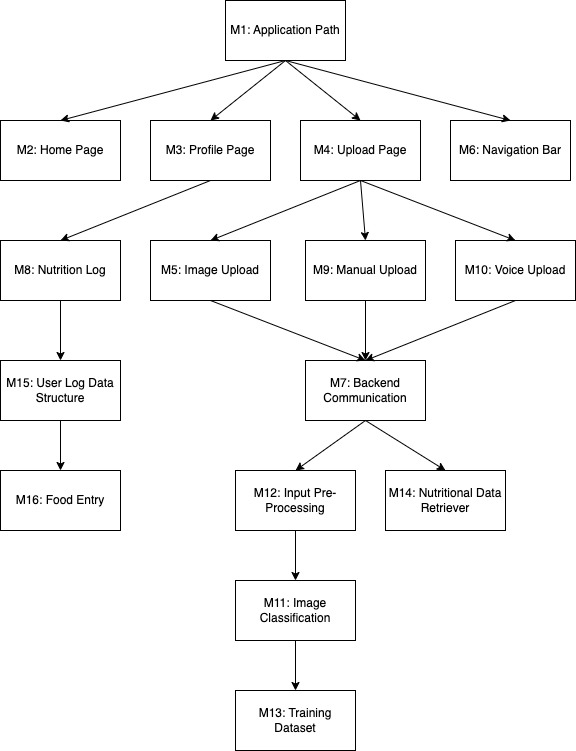
\includegraphics[width=0.7\textwidth]{use_hierarchy.png}
\caption{Use hierarchy among modules}
\label{FigUH}
\end{figure}

%\section*{References}

\bibliographystyle {plainnat}
\bibliography{../../../refs/References}

\newpage{}
\section*{Appendix --- Reflection}

The information in this section will be used to evaluate the team members on the
graduate attribute of Lifelong Learning.  Please answer the following questions:

\begin{enumerate}
  \item 
  \item 
\end{enumerate}

\end{document}
